\documentclass[10pt, a4paper]{article}
% The next line loads some packages you will need
\usepackage{graphicx, amsmath, amssymb, fancyhdr, setspace}
\usepackage[round]{natbib}
\usepackage{siunitx}
\usepackage{pgfplots}
\pgfplotsset{compat=1.11}
\usepackage{amsthm}
\usepackage{bm}
\usepackage{nicefrac}
\usepackage{hyperref}
\usepackage[noabbrev]{cleveref}
% Page formatting
\addtolength{\textwidth}{5mm}
\addtolength{\textheight}{12mm}
\addtolength{\topmargin}{-10mm}
\pretolerance = 10000000
\setlength{\parindent}{0pt}
\setlength{\parskip}{\baselineskip}
\onehalfspacing   
\newtheorem{exmp}{Example}[section]
\numberwithin{equation}{section}
\definecolor{color1}{RGB}{0,0,90} % Color of the article title and sections
\definecolor{color2}{RGB}{0,20,20} % Color of the boxes behind the abstract and headings
\hypersetup{hidelinks,colorlinks,breaklinks=true,urlcolor=color2,citecolor=color1,linkcolor=color1,bookmarksopen=false,pdftitle={Title},pdfauthor={Author}}
\newcommand{\rhob}{\bar{\rho}}
\newcommand{\srho}{\rhob + (\rho(\bm{x},t) -\rhob)}
\newcommand{\srhos}{\rhob + (\rho -\rhob)}
\newcommand{\DD}[2]{\frac{D#1}{D#2}}
\newcommand{\Dt}[1]{\DD{#1}{t}}
\newcommand{\vel}{\bm{u}}
\newcommand{\grav}{\bm{g}}
\newcommand{\del}{\nabla}
\newcommand{\deldot}{\nabla \cdot}
\newcommand{\delcross}{\nabla \times}
\newcommand{\inv}[1]{\frac{1}{#1}}
\newcommand{\bO}{\bm{\Omega}}
\newcommand{\bo}{\bm{\omega}}
\newcommand{\qv}{\bm{q}}
\newcommand{\delh}{\nabla_h}
\newcommand{\DDh}[2]{\frac{D_h#1}{D#2}}
\newcommand{\Dth}[1]{\DDh{#1}{t}}
\newcommand{\Dthexp}[1]{\partial_t {#1} + u \partial_x {#1} + v \partial_y {#1}}
\newcommand{\io}{\iota}
\newcommand{\ba}{\bm{A}}
\newcommand{\bb}{\bm{B}}
\newcommand{\bc}{\bm{C}}
% Header / footer
\pagestyle{fancy}
\lhead{Kieran Newman, 200901399}
\chead{}
\rhead{\em MATH 5825M, assignment 3}
\lfoot{}
\cfoot{\thepage}
\rfoot{}
\setlength{\headheight}{20pt}
\renewcommand{\headrulewidth}{0.4pt}
\renewcommand{\footrulewidth}{0pt}

\begin{document}
\begin{center}
\textbf{\Large Vortex Leapfrogging} \\
\end{center}
\section{Introduction}
Vortex interactions are an area of fluid dynamics still undergoing significant research.
In this piece of work, we will first explore the dynamics of vortices and their interactions, then analyse the stability of a system of four vortices, following the work by \citet{acheson00}.
A program was written in MATLAB to plot the paths of vortices in this system, and this is given in \hyperref[sec:ap1]{Appendix 1}.
\subsection{Notation}
\label{sec:notation}
Many differing notations are used in the literature for differential operators, vorticity, vectors and other terms. In this piece of work, the first partial derivative is represented by
\begin{equation}
\label{eq:1partial}
\frac{\partial}{\partial t} = \partial _t,
\end{equation}
and the second by
\begin{align}
\label{eq:doublepartial}
\frac{\partial^2}{\partial t^2} &:= \partial_{tt},\\
\label{eq:mixedpartial}
\frac{\partial^2}{\partial x\partial y} &:= \partial_{xy}
\end{align}
for double and mixed derivatives. Vectors are written
\begin{equation}
\label{eq:vector}
\bm{a}=\left(\begin{array}{c} a_1\\\vdots\\a_n \end{array}\right),
\end{equation}
and velocity is written (in three dimensional cartesian coordinates) as
\begin{equation}
\label{eq:veloc}
\vel=\left(\begin{array}{c} u_x\\u_y\\u_z \end{array}\right).
\end{equation}
\subsection{Vector Identities}
The following vector identities are used in this piece of work.
There is much use of the so-called ``Del'' operator, represented by (for Cartesian coordinates)
\begin{equation}
\label{eq:deldef}
\del=\left(\begin{array}{c} \partial_{x}\\\partial_{y}\\\partial_{z}\end{array}\right).
\end{equation}
In this notation, the divergence of a fluid is given by the inner product of ``Del'' with the velocity
\begin{equation}
\label{eq:divdef}
\mbox{div} (\vel) = \deldot \vel = \partial_x u_x + \partial_y u_y + \partial_z u_z,
\end{equation}
and the curl is given by the outer product
\begin{equation}
\label{eq:curldef}
\mbox{curl} (\vel) = \delcross \vel = \left(\begin{array}{c} \partial_y u_z -\partial_z u_y\\\partial_z u_x - \partial_x u_z\\\partial_x u_y - \partial_y u_x\end{array}\right).
\end{equation}
The triple outer product of $\vel$ and $\del$ can be written using the following identity (from \citet{harlen14c6})
\begin{equation}
\label{eq:vecid1}
\vel\times (\delcross \vel)=\inv{2}\del(\vel^2) -\vel\cdot\del\vel.
\end{equation}
\section{Dynamics of Vortices}
The general motion of a fluid is given by the Navier-Stokes equations, which are usually written in vector form:
\begin{equation}
\label{eq:navierstokes}
\partial_t\vel + \vel\cdot\del\vel = \nu \del^2 \vel -\inv{\rho} \del P,
\end{equation}
where $\rho$ is the fluid density, $P$ is the pressure and $\nu$ is the \emph{kinematic viscosity}, $\nicefrac{\mu}{\rho}$.
When working with incompressible fluids, we also use the continuity equation
\begin{equation}
\label{eq:cont}
\deldot \vel =0.
\end{equation}
This can be reworked to find an equation for the local vorticity of the fluid by remembering that the vorticity $\bo$ is equivalent to the vector curl of the velocity $\vel$.
Following \citet{harlen14c6}, we can rewrite \cref{eq:navierstokes} using the identity in \cref{eq:vecid1}
\begin{equation}
\label{eq:navs2}
\partial_t \vel + \inv{2}\del(\vel^2) - \vel\times (\delcross \vel) = \nu \del^2 \vel -\inv{\rho} \del P.
\end{equation}
Taking the curl of the whole equation, we obtain
\begin{equation}
\label{eq:veq1}
\partial_t \delcross\vel + \inv{2}\delcross(\del(\vel^2))-\delcross(\vel\times (\delcross \vel))=\delcross(\nu \del^2 \vel) -\delcross(\inv{\rho} \del P).
\end{equation}
Now rewriting in terms of $\bo$ and noting that the outer product of $\del$ with a gradient is zero always, many parts of \cref{eq:veq1} disappear and we are left with
\begin{equation}
\label{eq:veq2}
\partial_t \bo -\delcross(\vel\times\bo) = \nu \del^2 \bo.
\end{equation}
Using another expanded version of the triple vector product (again following \citet{harlen14c6})
\begin{equation}
\delcross(\vel \times \bo) = \vel\deldot\bo+\bo\cdot\del\vel -\bo\deldot\vel - \vel\cdot\del\bo,
\label{eq:vecid2}
\end{equation}
we can then write 
\begin{equation}
\partial_t \bo -  \vel\deldot\bo+\bo\cdot\del\vel -\bo\deldot\vel - \vel\cdot\del\bo = \nu \del^2 \bo.
\label{eq:veq3}
\end{equation}
However, from the continuity equation (\cref{eq:cont}) we have that $\deldot\vel=0$, and we also know that the divergence of a curl is always zero, so as $\bo=\delcross\vel$, $\deldot\bo=0$.
This means we can further rewrite \cref{eq:veq3} to obtain
\begin{equation}
\partial_t \bo + \vel\cdot \del\bo = \bo \cdot \del\vel + \nu \del^2 \bo,
\label{eq:veq4}
\end{equation}
the \emph{vorticity equation}.
When working in two dimensions only, which will be the situation for this piece of work, this equation reduces to a scalar equation in $\omega(x,y,t)$, the scalar vorticity (noting that the velocity $\vel$ and differential operator $\del$ are now two dimensional also)
\begin{equation}
\partial_t \omega + \vel \cdot \del \omega = \nu \del^2 \omega
\label{eq:2dveq}
\end{equation}
\citep{wayne11}.
Such vortices are known as \emph{Line Vortices}, comprising a central singularity with a circulation speed at distance $r$ of $\nicefrac{k}{r}$, for constant $k$, the vortex strength.
\subsection{Streamfunctions}
When considering line vortices in two dimensional, incompressible flow, it is generally simpler to use a \emph{streamfunction} to describe the fluid motion. 
We define a scalar function $\psi(x,y)$, known as the streamfunction, which is related to the fluid velocity via partial differentials
\begin{align}
\label{eq:sf1}
u_x=\partial_y \psi,\\
\label{eq:sf2}
u_y=-\partial_x \psi
\end{align}
\citep{harlen14c1}.
\section{Vortex Interactions}
In \citeyear{helmholtz67}, \citeauthor{helmholtz67} found that two vortices in the same plane (as in the two-dimensional flow we consider here) would each affect the other, with the form of the effect depending on the polarity and strength of each vortex.
\citeauthor{helmholtz67} described the interaction of two vortex ``rings'' ( toroidal vortex tubes in three dimensions \citep{saffman92}) as a ``game'', noting that, providing there was not too great a difference in the velocities of the vortices, they would travel together in the same direction with an oscillating motion.
This interaction can be thought of as the interaction of two smoke rings.
One ring shrinks, and passes through the other, before widening and slowing.
The second ring then shrinks, speeds up and passes through the first, before the cycle repeats again.
If a horizontal cross-section is taken through the toroid, and if the radius of the toroidal section (i.e. the radius of the vortex tube itself, not the ring radius) is taken infinitesimally small, the system becomes one of line vortices in a single plane. 
A single ring of diameter $\alpha$, centred at $y=0$, would represent as two line vortices at $\pm\alpha$, with the same strength but opposite polarity.
These two vortices would move in the $x$ direction together, as the ring would move in space, and this system can be shown by using the MATLAB code in \hyperref[sec:ap1]{Appendix 1}, with the following inputs:
\begin{verbatim}
EDU>> vortexleap
number of vortices = 2
number of time steps = 10000
step-size = 0.01
strength of vortex 1 = 1
strength of vortex 2 = -1
x-coordinate of vortex 1 = 0
y-coordinate of vortex 1 = 0.5
x-coordinate of vortex 2 = 0
y-coordinate of vortex 2 = -0.5
\end{verbatim}
giving \cref{fig:2vort}.
\begin{figure}[ht]
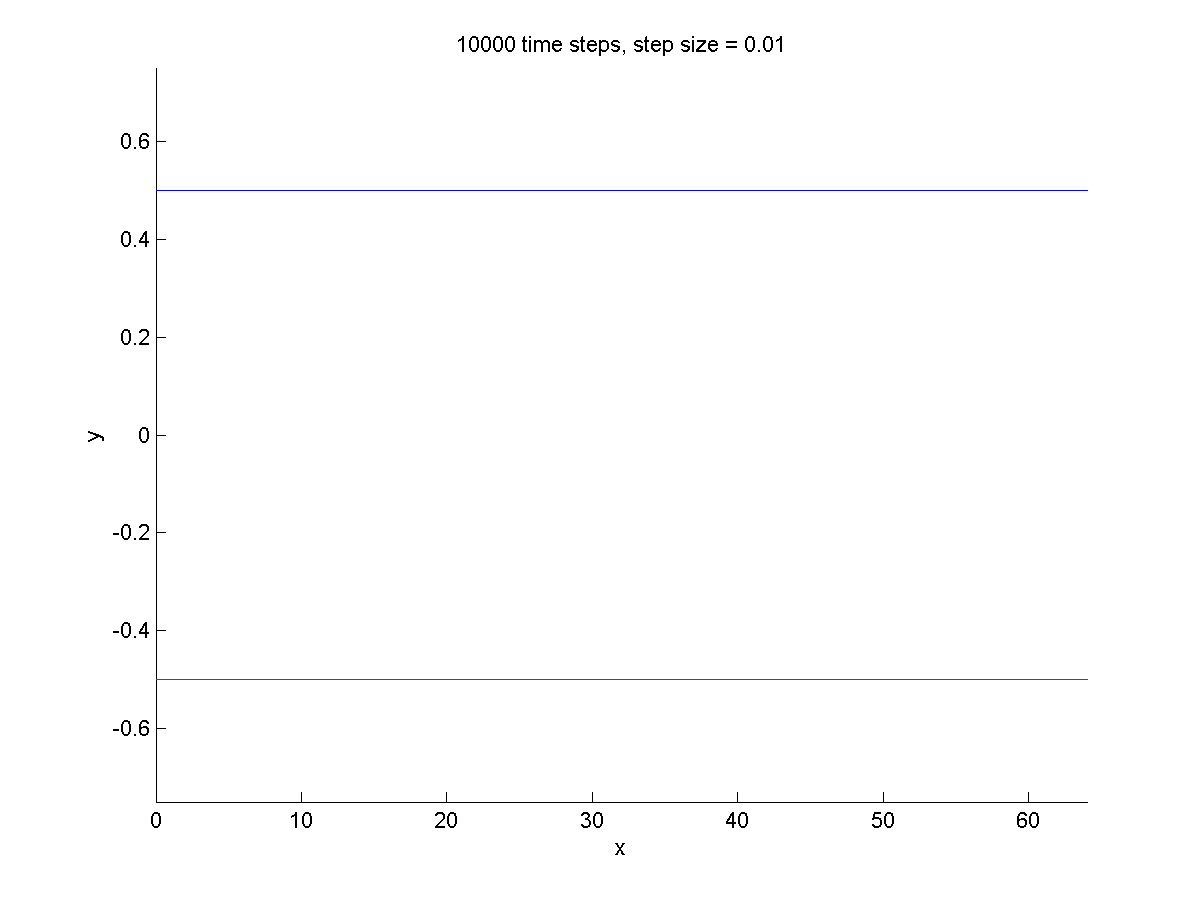
\includegraphics[width=\textwidth]{2vort}
\caption{Interaction of two line vortices of opposite polarity, representing a single vortex ring.}
\label{fig:2vort}
\end{figure}

The mentions of the two-ring interaction made by \citeauthor{helmholtz67} were not a detailed description of the motion of this system, and this was the basis for a paper by \citet{love94}.
\citeauthor{love94} modelled the system also as that of line vortices, with two pairs symmetrically arranged about the $x$ axis, with opposite polarity either side, as in \cref{fig:lovevort}.
\begin{figure}[ht]
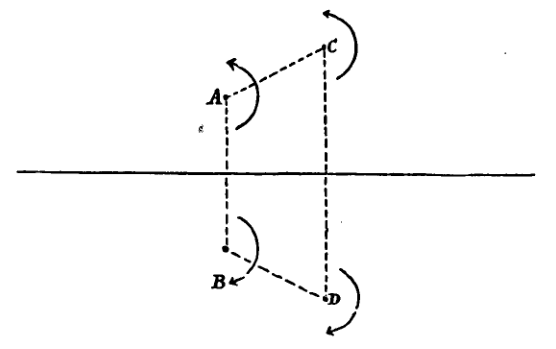
\includegraphics[width=\textwidth]{lovevort}
\caption{Point vortex pairs (A-B and C-D), from \citet[p.186]{love94}}
\label{fig:lovevort}
\end{figure}
If the vortex coordinates are
\begin{align}
\mbox{A:}&\hspace{0.5in}(x_0,y_0)\\
\mbox{B:}&\hspace{0.5in}(x_0,-y_0)\\
\mbox{C:}&\hspace{0.5in}(x_1,y_1)\\
\mbox{D:}&\hspace{0.5in}(x_1,-y_1)
\end{align}
and they have strengths $k$ (A and C) and $-k$ (B and D), then the motion of the fluid can be described by a streamfunction
\begin{equation}
\psi(x,y)=\frac{k}{2\pi}\ln\left(\frac{(x-x_0)^2 + (y+y_0)^2}{(x-x_0)^2 + (y-y_0)^2}\right) + \frac{k}{2\pi}\ln\left(\frac{(x-x_1)^2 + (y+y_1)^2}{(x-x_1)^2 + (y-y_1)^2}\right)
\label{eq:lovesf}
\end{equation}
\citep{love94}.

Now, with the aim of using the definitions of the streamfunction (\cref{eq:sf1,eq:sf2}), we differentiate \cref{eq:lovesf} with respect to $y$
\begin{align}
\partial_y \psi = \frac{k}{\pi}&\left(\frac{y+y_0}{(x-x_0)^2 + (y+y_0)^2}-\frac{y-y_0}{(x-x_0)^2 + (y-y_0)^2}\right.\nonumber\\&\left.+\frac{y+y_1}{(x-x_1)^2 + (y+y_1)^2}-\frac{y-y_1}{(x-x_1)^2 + (y-y_1)^2}\right),
\label{eq:lovesfdy}
\end{align}
and with respect to $x$
\begin{align}
\partial_x \psi = \frac{k}{\pi}&\left(\frac{x-x_0}{(x-x_0)^2 + (y+y_0)^2}-\frac{x-x_0}{(x-x_0)^2 + (y-y_0)^2}\right.\nonumber\\&\left.+\frac{x-x_1}{(x-x_1)^2 + (y+y_1)^2}-\frac{x-x_1}{(x-x_1)^2 + (y-y_1)^2}\right).
\label{eq:lovesfdx}
\end{align}
Now, we wish for the velocity of the vortices, i.e. we are looking at the above equations when $(x,y)\rightarrow(x_0,y_0)$ (or $(x_1,y_1)$).
Again following \citeauthor{love94}, we remove the terms that become infinite in this limit, thus obtaining,
\begin{alignat}{3}
\frac{dx_0}{dt}&=u_x (x_0,y_0)&&= \frac{k}{\pi} \left( \frac{y_1-y_0}{(x_0-x_1)^2 + (y_0-y_1)^2} + \frac{y_0+y_1}{(x_0-x_1)^2 +(y_0+y_1)^2} + \frac{1}{2y_0}\right),\label{eq:vortm1}\\
\frac{dy_0}{dt}&=u_y (x_0,y_0)&&= \frac{k}{\pi} \left( \frac{x_0-x_1}{(x_0-x_1)^2 + (y_0-y_1)^2} + \frac{x_1-x_0}{(x_0-x_1)^2 +(y_0+y_1)^2}\right),\label{eq:vortm2}\\
\frac{dx_1}{dt}&=u_x (x_1,y_1)&&= \frac{k}{\pi} \left( \frac{y_0-y_1}{(x_1-x_0)^2 + (y_1-y_0)^2} + \frac{y_1+y_0}{(x_1-x_0)^2 +(y_1+y_0)^2} + \frac{1}{2y_1}\right),\label{eq:vortm3}\\
\frac{dy_1}{dt}&=u_y (x_1,y_1)&&= \frac{k}{\pi} \left( \frac{x_1-x_0}{(x_1-x_0)^2 + (y_1-y_0)^2} + \frac{x_0-x_1}{(x_1-x_0)^2 +(y_1+y_0)^2} \right).\label{eq:vortm4}
\end{alignat}

\citet{acheson00} generalised these equations for a system of $N$ vortices (with strengths $k_1,k_2,\ldots ,k_N$), obtaining
\begin{align}
\frac{dx_i}{dt}&=\sum^N_{\substack{j=1\\j\neq i}} k_j \frac{y_j - y_i}{(x_i - x_j)^2 + (y_i - y_j)^2},\label{eq:vortposx}\\
\frac{dy_i}{dt}&=\sum^N_{\substack{j=1\\j\neq i}} k_j \frac{x_i - x_j}{(x_i - x_j)^2 + (y_i - y_j)^2},\label{eq:vortposy}
\end{align}
for $i=1,2,\ldots, N$.
The summations in \cref{eq:vortposx,eq:vortposy} are implemented in \hyperref[vortexf]{\texttt{vortexf.m}} and \hyperref[vortexg]{\texttt{vortexg.m}} respectively.
\clearpage
\section*{Appendix I: MATLAB Code}\label{sec:ap1}
MATLAB code for the vortex leapfrogging program (\texttt{vortexleap.m}\normalfont) and subroutines (\texttt{vortexf.m}\normalfont,\texttt{vortexg.m}) are given below.
\subsection*{\texttt{vortexf.m}}
\label{vortexf}
\begin{verbatim}
function[fi]=vortexf(i,k,x,y,N)
fi=0;
jmat=[1:1:N];
jmat(i)=[];
for j=jmat
    rr=((x(i)-x(j))^2)+((y(i)-y(j))^2);
    fi=fi+(k(j)*(y(j)-y(i))/rr);
end
end
\end{verbatim}
\subsection*{\texttt{vortexg.m}}
\label{vortexg}
\begin{verbatim}
function[gi]=vortexg(i,k,x,y,N)
gi=0;
jmat=[1:1:N];
jmat(i)=[];
for j=jmat
    rr=((x(i)-x(j))^2)+((y(i)-y(j))^2);
    gi=gi+(k(j)*(x(i)-x(j))/rr);
end
end
\end{verbatim}
\subsection*{\texttt{vortexleap.m}}
\label{vortexleap}
\begin{verbatim}
clear all
N=input('number of vortices = ');
%set time step and scales
t=0;
T=input('number of time steps = ');
%set length step and scales
h=input('step-size = ');
%define vortex strengths
for i=1:N
    k(i)=input(['strength of vortex ',num2str(i),' = ']);
end
%define variable for position
x=NaN(1000,N);
y=NaN(1000,N);
for i=1:N
    x(1,i)=input(['x-coordinate of vortex ',num2str(i),' = ']);
    y(1,i)=input(['y-coordinate of vortex ',num2str(i),' = ']);
end
for a=2:T
    clear x1 x2 x3 x4 y1 y2 y3 y4 k1 k2 k3 k4 l1 l2 l3 l4
    x1=x(a-1,:);
    y1=y(a-1,:);
    k1=NaN(1,N);
    k2=NaN(1,N);
    k3=NaN(1,N);
    k4=NaN(1,N);
    l1=NaN(1,N);
    l2=NaN(1,N);
    l3=NaN(1,N);
    l4=NaN(1,N);
    for i=1:N
        k1(i)=h*vortexf(i,k,x1,y1,N);
        l1(i)=h*vortexg(i,k,x1,y1,N);
    end
    x2=x1+(k1/2);
    y2=y1+(y1/2);
    for i=1:N
        k2(i)=h*vortexf(i,k,x2,y2,N);
        l2(i)=h*vortexg(i,k,x2,y2,N);
    end
    x3=x1+(k2/2);
    y3=y1+(y2/2);
    for i=1:N
        k3(i)=h*vortexf(i,k,x3,y3,N);
        l3(i)=h*vortexg(i,k,x3,y3,N);
    end
    x4=x1+(k3);
    y4=y1+(y3);
    for i=1:N
        k4(i)=h*vortexf(i,k,x4,y4,N);
        l4(i)=h*vortexg(i,k,x4,y4,N);
    end
    x(a,:)=x(a-1,:)+((1/6)*(k1+2*k2+2*k3+k4));
    y(a,:)=y(a-1,:)+((1/6)*(l1+2*l2+2*l3+l4));
    percent=100*a/T;
    display([num2str(percent),'% done'])
end
clf
%for viewing evolution of tracks
%multicomet(x,y)
%for viewing static image of tracks
colourmap=['b','r','g','c','m','y','k'];
maxy=1.5*max(max(abs(y)));
hold on
for i=1:N
    plot(x(:,i),y(:,i),colourmap(i))
end
xlabel('x');
ylabel('y');
title([num2str(T),' time steps, step size = ',num2str(h)]);
axis([0 inf -maxy maxy])
hold off
name=input('file name? ');
print('-dpng',[name,'.png']);
\end{verbatim}
The scheme used is a fourth order Runge-Kutta method with non-adaptive step size. The equations plotted are from \citet{acheson00}.
\bibliographystyle{dcu}
\bibliography{kwnrefs}
\end{document}
